%!TEX root = ./trampoline.tex



%% HEAD SUPERTABULAR %%
\rowcolors{1}{light-gray}{white}
\newlength{\Li}\settowidth{\Li}{\textbf{Decimal}}
\newlength{\Liii}\settowidth{\Liii}{(bootstrap  )}
\newlength{\Lii}\settowidth{\Lii}{SCHEDULETABLE_AUTOSTART }
\tablefirsthead{ \textbf{Decimal Value} & \textbf{bit 5}  & \textbf{bit 4} & \textbf{bit 3} & \textbf{bit 2} & \textbf{bit 1} & \textbf{bit 0} & \textbf{Meaning} \\ \hline }
\tablehead{ \rowcolor{white} \rowcolors{1}{light-gray}{white} \textbf{Decimal Value} & \textbf{bit 5}  & \textbf{bit 4} & \textbf{bit 3} & \textbf{bit 2} & \textbf{bit 1} & \textbf{bit 0} & \textbf{Meaning} \\ \hline  }
\tabletail{ \hline } 
\tablelasttail{}


\chapter{Schedule Table Implementation}

Here is the files list :
\begin{itemize}
\item \file{tpl_as_schedtable.c} contains the API services.
\item \file{tpl_as_st_kernel.c} contains the kernel API services, \function{tpl_process_schedtable()} and \function{tpl_adjust_next_expiry_point()}
\item \file{tpl_as_action.c} contains \function{tpl_action_finalize_schedule_table()}
\item \file{tpl_as_definitions.h} contains the schedule table's states (SCHEDULETABLE\_STOPPED, SCHEDULETABLE\_BOOTSTRAP, SCHEDULETABLE\_AUTOSTART\_ABSOLUTE...)
\item \file{tpl_os_timeobj_kernel.c} contains \function{tpl_remove_time_obj()} which has been modified for the schedule table object.
\end{itemize}

The schedule table class diagram is shown in Figure \ref{fig:STobject} below.

\begin{figure}[H] %  figure placement: here, top, bottom, or page
   \centering
   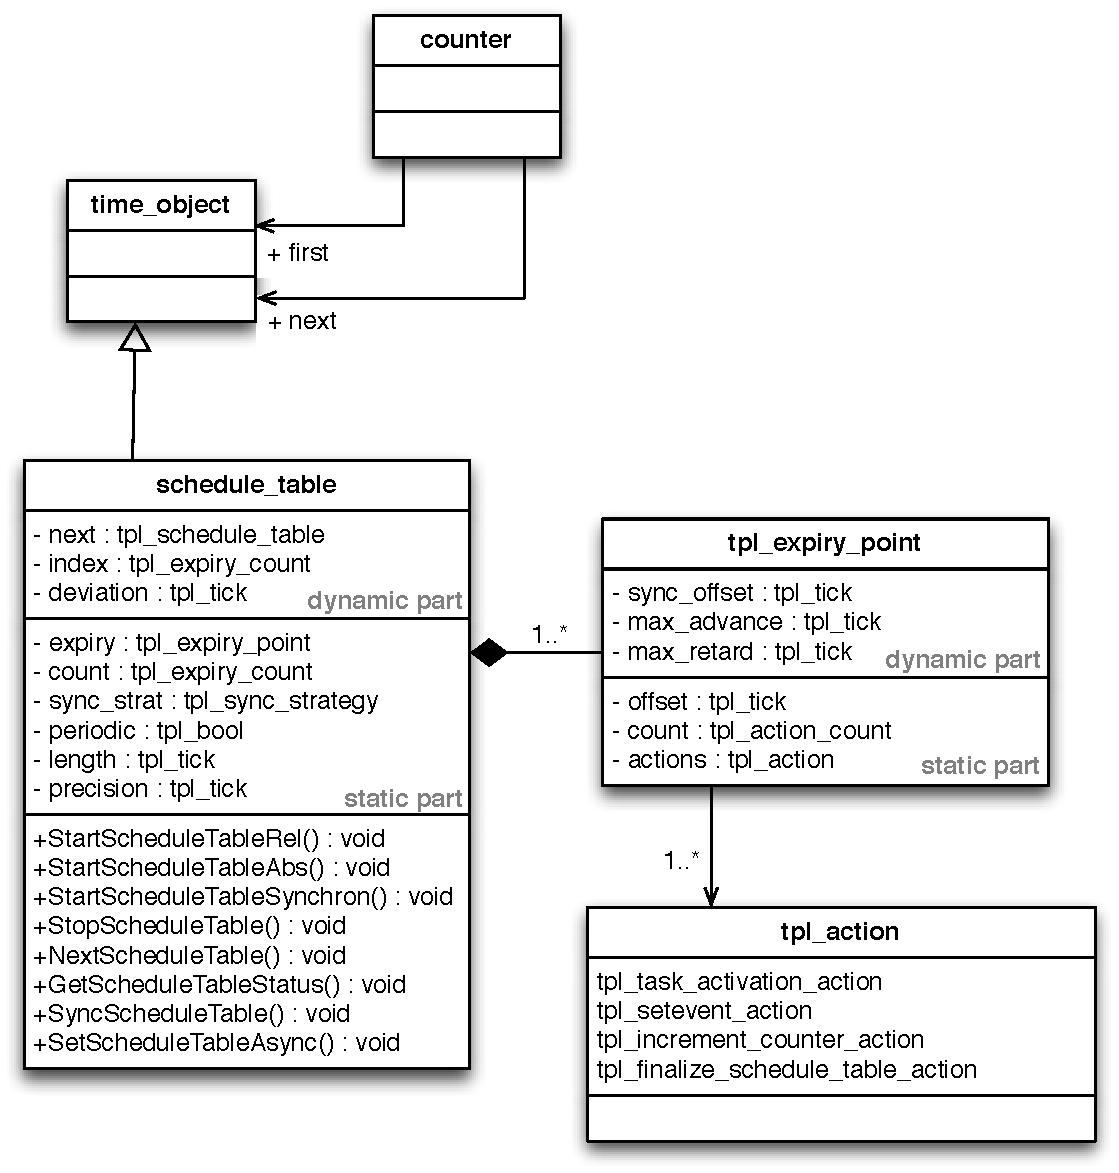
\includegraphics[scale=0.6]{pictures/STobject.pdf}  
   \caption{Schedule table class diagram}
   \label{fig:STobject}
\end{figure} 



\section{The States of a Schedule Table}

A schedule table always has a defined state. States include those found at page 42 of the AUTOSAR specifications 3.1 and others states used for internal management.

Indeed, \textbf{bit 1} is the "autostart" bit. It's used when autostarted schedule tables have been declared in the OIL file. Goil generates schedule tables with SCHEDULETABLE\_AUTOSTART\_X (X can be RELATIVE, ABSOLUTE or SYNCHRON) state. At startup (in \function{tpl_init_os()}), the system starts autostarted schedule tables and resets the \textbf{bit 1}.

\textbf{bit 4} is the "bootstrap" bit. It's used when the first expiry point of a schedule table is dated in more than \textbf{OsCounterMaxAllowedValue} ticks from the current date\footnote{As the \toreplace{offset} parameter of StartScheduleTableRel() cannot be greater than \textbf{OsCounterMaxAllowedValue} minus the \textbf{InitialOffset} of the schedule table (OS276), the first expiry point cannot be in more than \textbf{OsCounterMaxAllowedValue} ticks from the current date. Thus the "bootstrap" bit can set by StartScheduleTableAbs() only.}. It can happen when :
	\begin{itemize}
	\item the schedule table start (\toreplace{tick_val}) is after the current date and the first expiry point comes between the current date and \toreplace{tick_val}
	\item \toreplace{tick_val} is before the current date and the first expiry point comes after the current date
	\end{itemize}

Figure \ref{fig:bootstrapexample} below shows a bootstrap example for the first item.

\begin{figure}[H] %  figure placement: here, top, bottom, or page
   \centering
   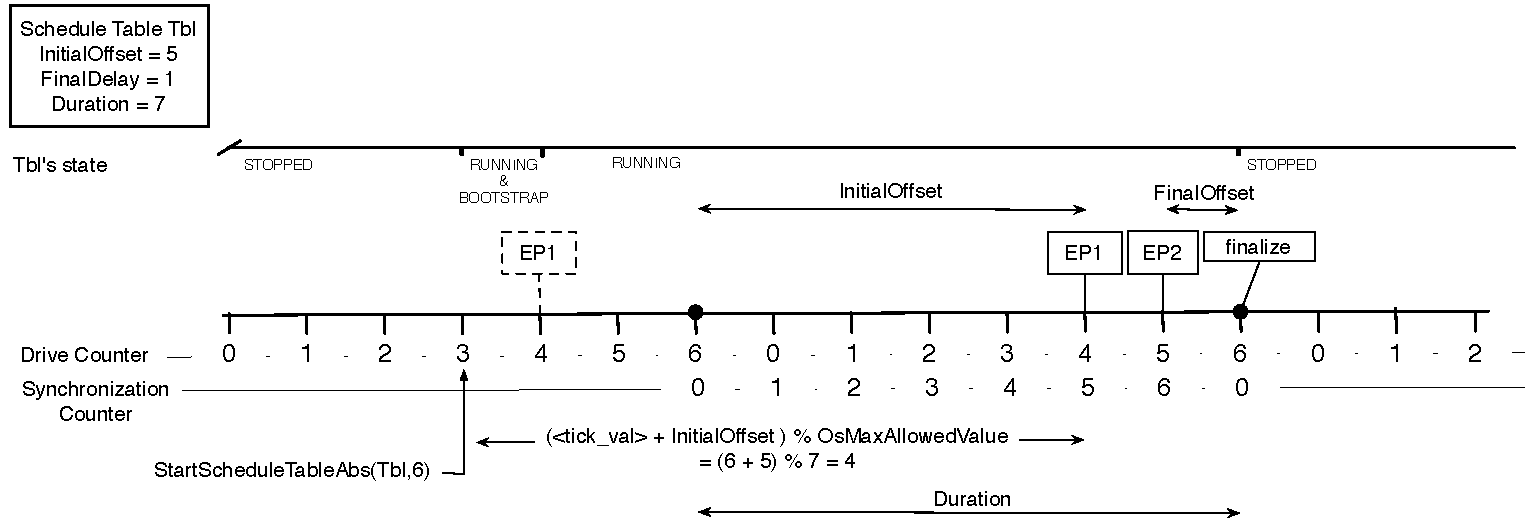
\includegraphics[scale=0.6]{pictures/BootstrapExample.pdf}  
   \caption{Bootstrap example}
   \label{fig:bootstrapexample}
\end{figure} 

\textbf{bit 5} is the "asynchronous" bit. It tells the system that the schedule table is in asynchronous mode.\\
Thus, the different states of a schedule table are described in Table \ref{schedtablestates} below.


\begin{table}[H]
\begin{center}
\topcaption{\textcolor{white}{q}States of a schedule table } % Latex is weird, the table goes on the next page without the "\textcolor{white}{q}"
\begin{supertabular}{p{\Li}|c|c|c|c|c|c|p{\Lii}|} 
0	& 0	& 0	& 0 	& 0	& 0	& 0	& SCHEDULETABLE_STOPPED  \\ 
1	& 0	& 0	& 0 	& 0	& 0	& 1	& SCHEDULETABLE_RUNNING  \\ 
5	& 0	& 0	& 0 	& 1	& 0	& 1	& SCHEDULETABLE_NEXT  \\  
9	& 0	& 0	& 1 	& 0	& 0	& 1	& SCHEDULETABLE_WAITING  \\  
13	& 0	& 0	& 1 	& 1	& 0	& 1	& SCHEDULETABLE_RUNNING_AND_SYNCHRONOUS \\ \hline \hline
6	& 0	& 0	& 0 	& 1	& 1	& 0	& SCHEDULETABLE_AUTOSTART _ABSOLUTE  \\ 
10	& 0	& 0	& 1 	& 0	& 1	& 0	& SCHEDULETABLE_AUTOSTART _RELATIVE  \\  
14	& 0	& 0	& 1 	& 1	& 1	& 0	& SCHEDULETABLE_AUTOSTART _SYNCHRON  \\  \hline \hline
16	& 0	& 1	& 0 	& 0	& 0	& 0	& SCHEDULETABLE_BOOTSTRAP \\ 
32	& 1	& 0	& 0 	& 0	& 0	& 0	& SCHEDULETABLE_ASYNC  \\ 
\end{supertabular} 
\end{center}
\label{schedtablestates}
\end{table}

Figure \ref{fig:STstates} shows how a schedule table goes from state to state.

\begin{figure}[H] %  figure placement: here, top, bottom, or page
   \centering
   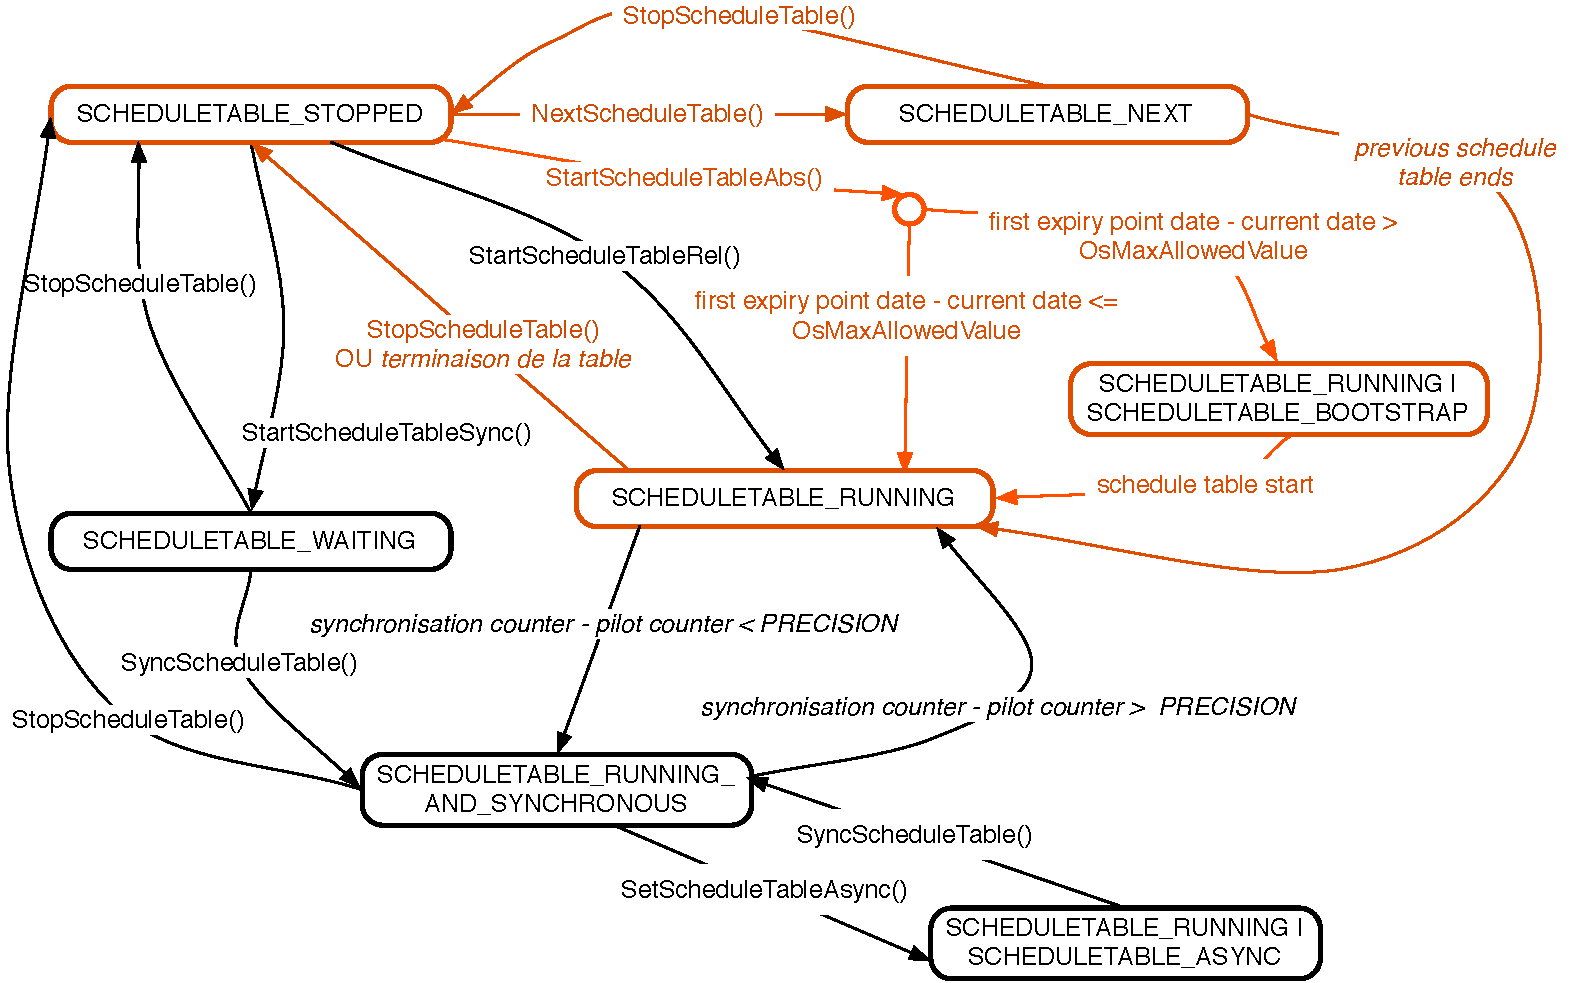
\includegraphics[scale=0.6]{pictures/STstates.pdf}  
   \caption{States of a schedule table in Trampoline.}
   \label{fig:STstates}
\end{figure} 
	
\section{Processing a Schedule Table}

In the same time of producing the schedule tables expiry points, GOIL adds one expiry point more than the number of expiry point delared in the OIL file : the "finalize" expiry point (see Figure \ref{fig:bootstrapexample}). Indeed, the RUNNING state of a "nexted" schedule table should be set at the finalize expiry point, thus, this expiry point has to be inserted. Moreover, for a periodic schedule table, the "finalize" expiry point helps to launch the first expiry point of the next period.

To process a \textbf{synchronized} schedule table, the schedule table's state has to be updated each expiry point and the next expiry point has to be adjusted according to the schedule table's deviation each epiry point too.

A schedule table is a time object, like an alarm. \function{tpl_processing_scheduletable()} is called by each expiry point (before activating a task, setting an event or finalizing a schedule table via \function{tpl_finalize_expiry_point()}) . The state machine of this function is shown in the Figure \ref{fig:STprocessingTplProcess}.

\begin{figure}[H] %  figure placement: here, top, bottom, or page
   \centering
   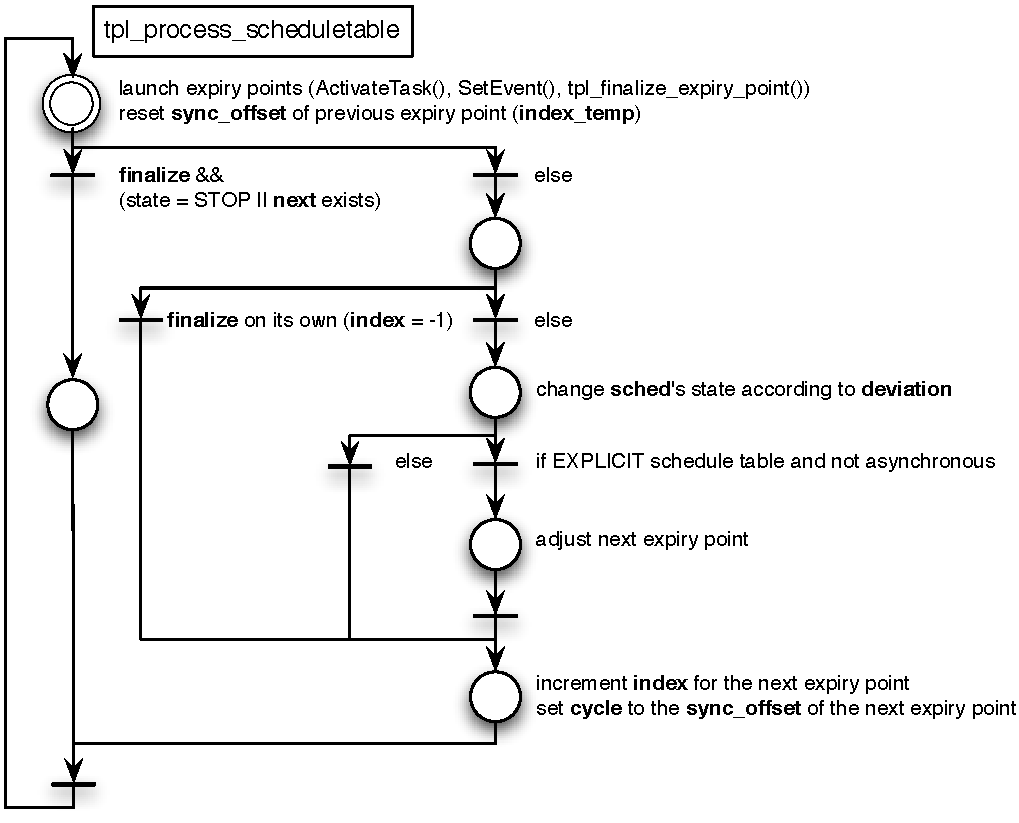
\includegraphics[scale=0.6]{pictures/STprocessingTplProcess.pdf}  
   \caption{tpl_process_scheduletable's state machine.}
   \label{fig:STprocessingTplProcess}
\end{figure} 

\begin{figure}[H] %  figure placement: here, top, bottom, or page
   \centering
   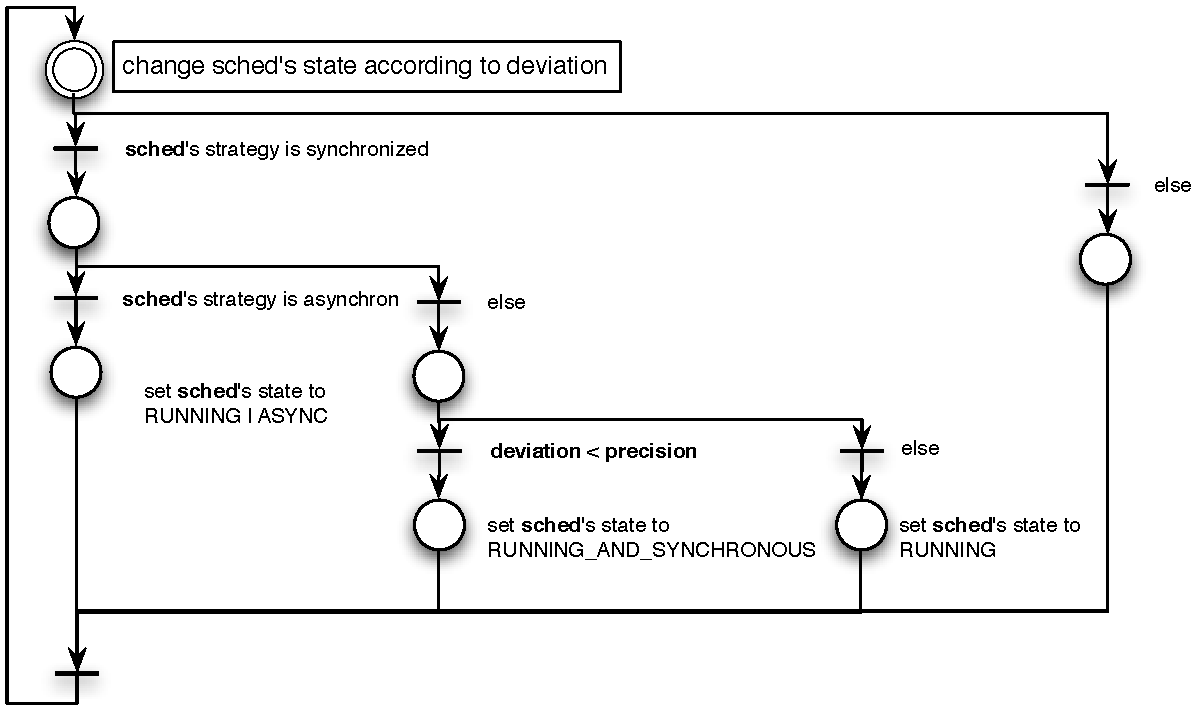
\includegraphics[scale=0.6]{pictures/STprocessingChangeState.pdf}  
   \label{fig:STprocessingChangeState}
\end{figure}

\begin{figure}[H] %  figure placement: here, top, bottom, or page
   \centering
   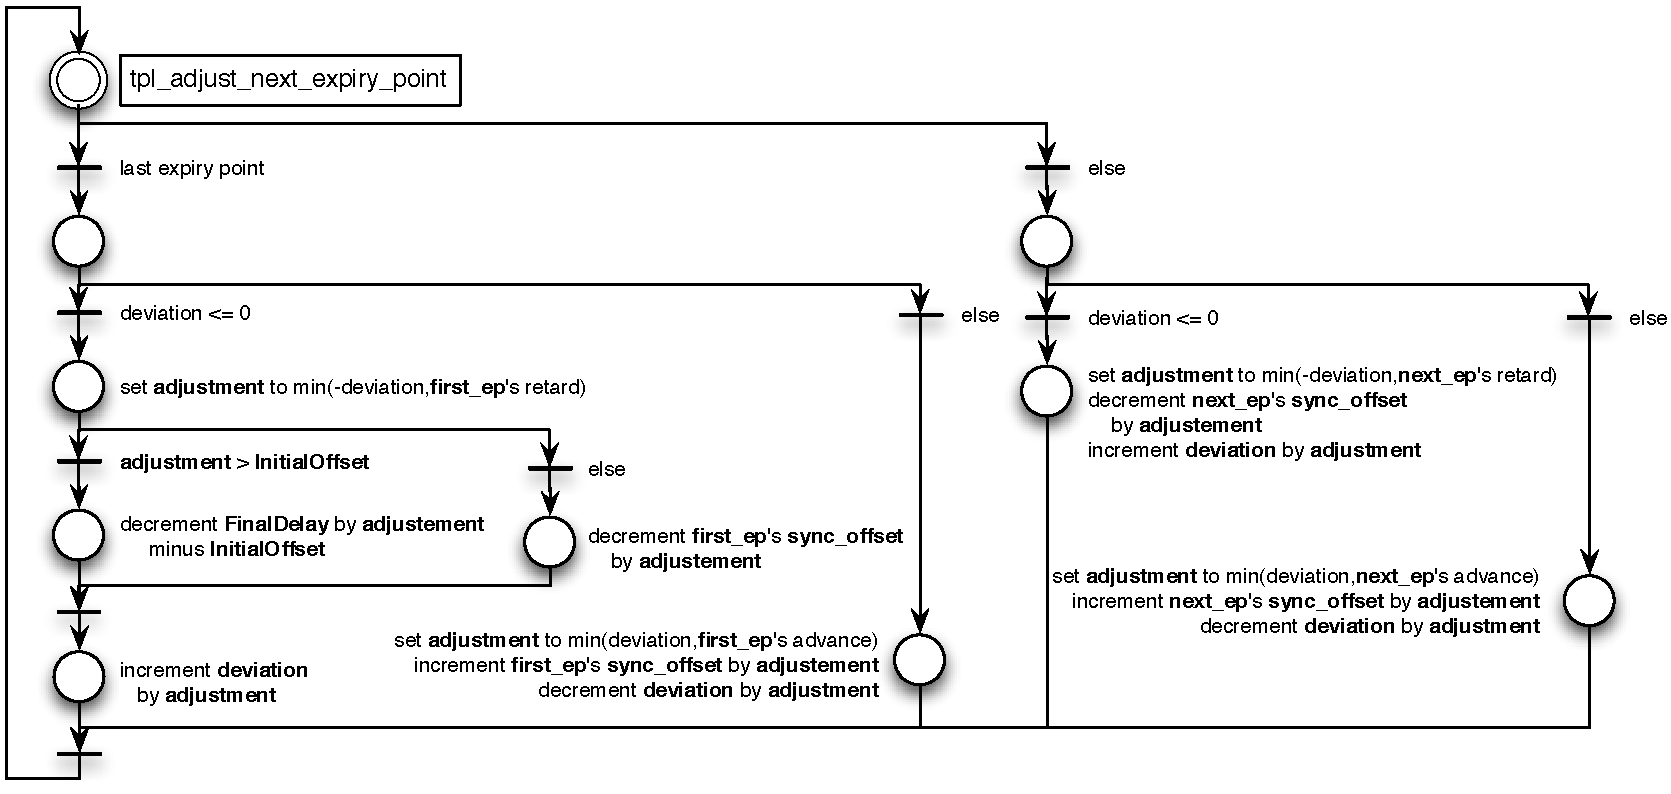
\includegraphics[scale=0.6]{pictures/STprocessingTplAdjust.pdf}  
   \label{fig:STprocessingTplAdjust}
\end{figure}

\function{tpl_finalize_expoiry_point()} state machine is shown in Figure \ref{fig:STprocessingTplFinalize} below.

\begin{figure}[H] %  figure placement: here, top, bottom, or page
   \centering
   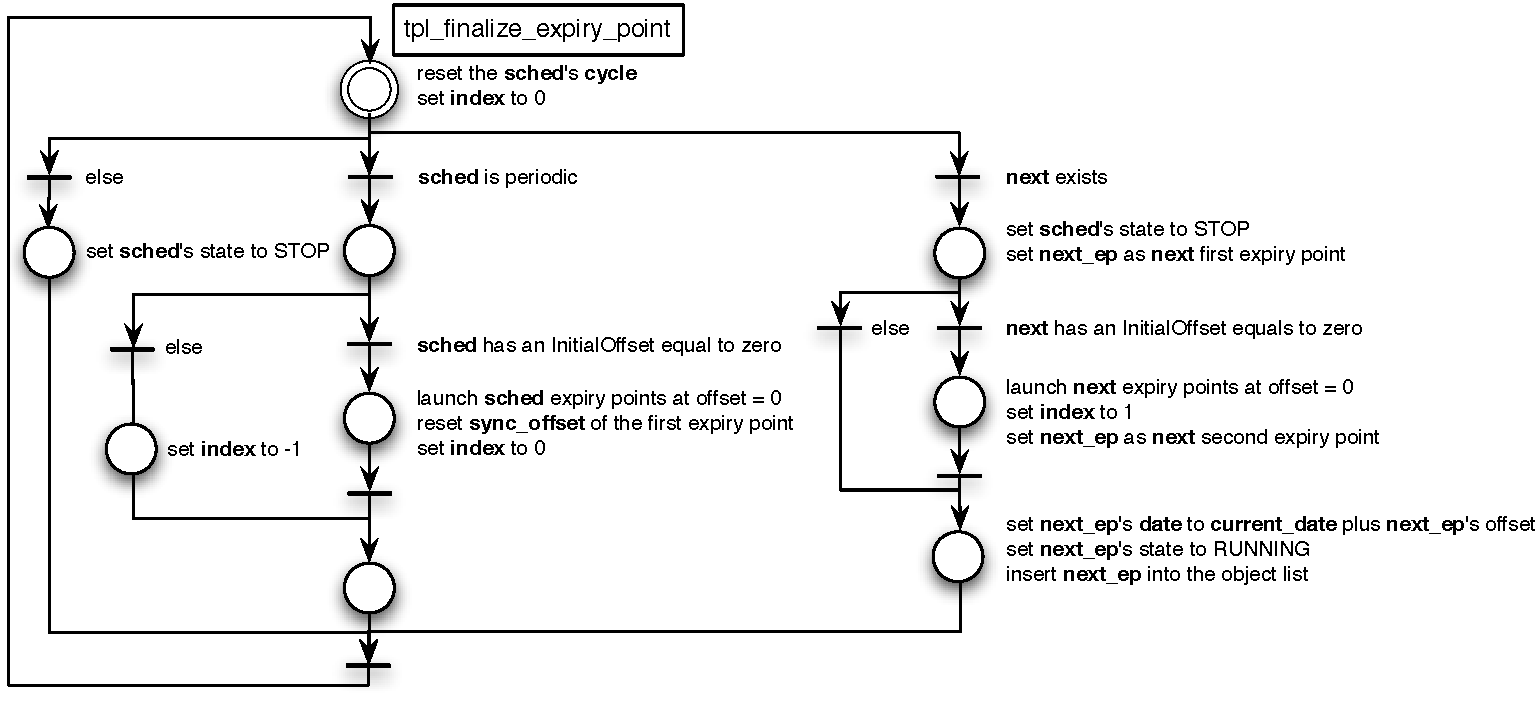
\includegraphics[scale=0.6]{pictures/STprocessingTplFinalize.pdf}  
   \caption{tpl_finalize_expiry_point's state machine.}
   \label{fig:STprocessingTplFinalize}
\end{figure} 
















